\section{Lagrange points analysis}
\label{sec:lagrange-points-analysis}

Lagrangian points are a set of special locations in the vicinity of two massive
bodies where a small object will maintain a relatively stable position relative
to the two massive bodies. The five Lagrange points are labeled L1 through L5.
L1, L2, and L3 are collinear with the two massive bodies, while L4 and L5 are
located at the vertices of the equilateral triangle formed by the two massive
bodies. The L1, L2, and L3 points are unstable, while L4 and L5 are stable. The
L4 and L5 points are sometimes called Trojan points, and the two massive bodies
are sometimes called the primaries. Figure \ref{fig:lagrange_points} shows the
Lagrange points in the Sun - Earth-Moon barycenter system.

Despite L1, L2, and L3 being unstable, they are of particular interest because
of their proximity to the primaries. In fact, stable orbits can be achieved
by performing small corrections to the spacecrafts's position. Also, these
points are not populated with asteroids like L4 and L5, making them excellent
for long term missions.

In this work, only the point L2 belonging to the Sun - Earth system is
considered. The reason for choosing this point is that it is a popular point
chosed by different missions and thus, a well known point. It provides a great
viewpoint. In fact, this point has been selected for other missions including
the James Webb Space Telescope, see \cite{gardner2006}, or the future Comet
Interceptor, see \cite{jones2019}.

\begin{figure}[H]
    \centering
    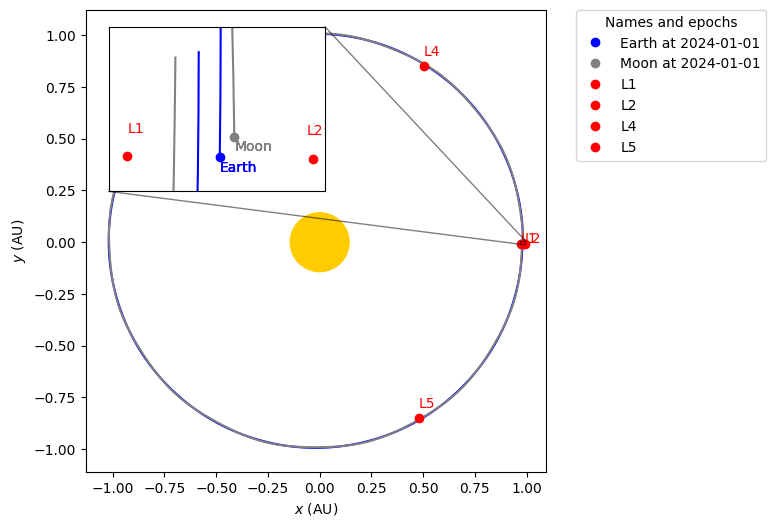
\includegraphics[width=\textwidth]{static/lagrange_points.png}
    \caption[Lagrange points in the Sun - Earth system.]{Lagrange points in the
        Sun - Earth-Moon barycenter system. All points are shown except L3. Ephemerides for this
        point are not provided by the JPL Horizons system. Despite this
        situation, the point is not analyzed in this work.}
    \label{fig:lagrange_points}
\end{figure}

\subsection{Escape velocity from L2}

For the computation of the escape velocity in the vicinity of the Lagrange
points, the gravitation effects of the Earth and the Moon are considered. Even
if the Lagrange points only appear in the restricted three-body problem,
computing the escape velocity requires using the two-body problem is still a
valid approach as long as the barycenter of the Earth-Moon system is used.

Thus, the escape velocity can be computed using equation \ref{eq:escape_velocity}.

\begin{equation}
        v_{\text{esc}} = \sqrt{\frac{2 \mu}{d}} = \sqrt{\frac{2 \mu}{\norm{\vec{r_b} - \vec{r}}}}
\label{eq:escape_velocity}
\end{equation}

where in $\mu$ is the gravitational parameter of the Earth-Moon system, and $d$
is the distance from the point of interest to the barycenter of the Earth-Moon
system, which can be computed using equation \ref{eq:earth_moon_distance}.

\begin{equation}
        \vec{r_{b}} = \frac{\vec{r_{\text{\Terra}}} \cdot m_{\text{\Terra}}
        + \vec{r_{\text{\Moon}}} \cdot m_{\text{\Moon}}}{m_{\text{\Terra}} +
        m_{\text{\Moon}}}
    \label{eq:earth_moon_distance}
\end{equation}

To simplify the computer routines, an average value for the escape velocity has
been computed by solving previous equations for a span of time ranging between
years 2000 and 2050. The mean value for the escape velocity from L2 is $0.73$
km/s.

\subsection{Optimum direct transfers from L2}

The analysis for a direct optimum transfer from L2 to each one of the discovered
ISOs follows the same model than the one presented in chapter
\ref{ch:direct-transfer}.

\subsubsection{'Oumuamua}

Figures \ref{fig:l2-oumuamua-optimum-porkchop} and
\ref{fig:l2-oumuamua-optimum-porkchop-avl} show the porkchop plots showing the
launch energy, time of flight, and arrival velocity for a direct prograde launch
between L2 and 'Oumuamua.

\begin{figure}[H]
  \centering
  \includegraphics[width=\textwidth]{static/oumuamua/l2-direct-detailed-porkchop-tof.png}
        \caption[Detailed porkchop showing the optimum transfer for
        L2 to 1I/'Oumuamua with the time of flight.]{Detailed porkchop showing the optimum transfer for
        L2 to 1I/'Oumuamua. 
  }
  \label{fig:l2-oumuamua-optimum-porkchop}
\end{figure}

Note that these figures are very similar to the ones in
\ref{fig:oumuamua-optimum-porkchop} and \ref{fig:oumuamua-optimum-porkchop-avl}.
The main difference is that launching from L2 requires less fuel, since the
escape velocity is lower. The required launch energy reduces about 92.81\%.
Despite this advantage, the arrival velocity is still high. Launch and arrival
dates are shown in table \ref{tab:l2-oumuamua-direct-transfer-optimum}.

\begin{figure}[H]
  \centering
  \includegraphics[width=\textwidth]{static/oumuamua/l2-direct-detailed-porkchop-avl.png}
        \caption[Detailed porkchop showing the optimum transfer for
        L2 to 1I/'Oumuamua with the arrival velocity.]{Detailed porkchop showing the
        optimum transfer for L2 to 1I/'Oumuamua with isolines for the arrival
        velocity.}
  \label{fig:l2-oumuamua-optimum-porkchop-avl}
\end{figure}

\vspace{1cm}
\begin{table}[H]
  \centering
  \begin{tabular}{|c|c|c|c|}
    \hline
    Object & Launch date & Arrival date & Required $C_3$ [km$^2$/s$^2$] \\
    \hline
    1I/'Oumuamua & 2017-01-22 & 2017-10-13 & 14.41 \\
    \hline
  \end{tabular}
  \caption[Optimum transfer orbit for a direct transfer between L2 and
        1I/'Oumuamua.]{Optimum transfer orbit for a direct transfer between
        L2 and 1I/'Oumuamua. The energy includes the required impulse for
        escaping the L2 point and for performing a targeting maneuver.}
  \label{tab:l2-oumuamua-direct-transfer-optimum}
\end{table}

The optimum transfer orbit is found to have a time of flight $\Delta t = 263.67$
days. The total cost of the launch is $\Delta v_\text{launch} = \Delta v_e +
\Delta v_1 = 0.73 \text{ km/s} + 3.07 \text{ km/s} = 3.80$ km/s. The arrival
impulse is $\Delta v_2 = 61.46$ km/s. If the rendezvous is considered, the total
cost of the maneuver adds up to $\Delta v = 64.53$ km/s. Detailed impulses are
shown in table \ref{tab:l2-oumuamua-direct-transfer-impulses}.

\vspace{1cm}
\begin{table}[H]
  \centering
  \begin{tabular}{|c|c|c|c|}
    \hline
    Impulse & $\Delta v_x$ [km/s] & $\Delta v_y$ [km/s] & $\Delta v_z$ [km/s] \\
    \hline
    Launch & 1.67 & -1.30 & 2.21 \\
    \hline
    Arrival & 58.04 & -14.06 & 14.47 \\
    \hline
  \end{tabular}
    \caption[Required impulses for a direct prograde transfer between L2 and
    'Oumuamua]{Required impulses for a direct prograde transfer between L2 and
    'Oumuamua.}
  \label{tab:l2-oumuamua-direct-transfer-impulses}
\end{table}


\subsubsection{Borisov}

Figures \ref{fig:l2-borisov-optimum-porkchop} and
\ref{fig:l2-borisov-optimum-porkchop-avl} show the porkchop plots showing the
launch energy, time of flight, and arrival velocity for a direct prograde launch
between L2 and Borisov.

\begin{figure}[H]
  \centering
  \includegraphics[width=\textwidth]{static/borisov/l2-direct-detailed-porkchop-tof.png}
        \caption[Detailed porkchop showing the optimum transfer for
        L2 to 2I/Borisov with the time of flight.]{Detailed porkchop showing the optimum transfer for
        L2 to 2I/Borisov. A point under 50 km$^2$/s$^2$ is found, highly
        reducing the launch cost from this Lagrange point.
  }
  \label{fig:l2-borisov-optimum-porkchop}
\end{figure}

\begin{figure}[H]
  \centering
  \includegraphics[width=\textwidth]{static/borisov/l2-direct-detailed-porkchop-avl.png}
        \caption[Detailed porkchop showing the optimum transfer for
        L2 to 2I/Borisov with the arrival velocity.]{Detailed porkchop showing the
        optimum transfer for L2 to 2I/Borisov with isolines for the arrival
        velocity. The optimum transfer point is found to have an arrival speed
        close to 33 km/s.}
  \label{fig:l2-borisov-optimum-porkchop-avl}
\end{figure}

Again, these figures are very similar to the ones in
\ref{fig:borisov-optimum-transfer-porkchop-tof} and
\ref{fig:borisov-optimum-transfer-porkchop-avl}. Again, launching from L2
requires less fuel. The required launch energy reduces about 88.08\%, yet the
arrival velocity is still high. Launch and arrival dates are shown in table
\ref{tab:l2-borisov-direct-transfer-optimum}.

\vspace{1cm}
\begin{table}[H]
  \centering
  \begin{tabular}{|c|c|c|c|}
    \hline
    Object & Launch date & Arrival date & Required $C_3$ [km$^2$/s$^2$] \\
    \hline
    2I/Borisov & 2018-07-12 & 2019-10-26 & 34.30 \\
    \hline
  \end{tabular}
  \caption[Optimum transfer orbit for a direct transfer between L2 and
        2I/Borisov.]{Optimum transfer orbit for a direct transfer between
        L2 and 2I/Borisov. The energy includes the required impulse for
        escaping the L2 point and for performing a targeting maneuver.}
  \label{tab:l2-borisov-direct-transfer-optimum}
\end{table}

The optimum transfer orbit is found to have a time of flight $\Delta t = 470.79$
days. The total cost of the launch is $\Delta v_\text{launch} = \Delta v_e +
\Delta v_1 = 0.73 \text{ km/s} + 5.13 \text{ km/s} = 5.83$ km/s. The arrival
impulse is $\Delta v_2 = 33.02$ km/s. If the rendezvous is considered, the total
cost of the maneuver adds up to $\Delta v = 38.85$ km/s. Detailed impulses are
shown in table \ref{tab:l2-borisov-direct-transfer-optimum}.

\vspace{1cm}
\begin{table}[H]
  \centering
  \begin{tabular}{|c|c|c|c|}
    \hline
    Impulse & $\Delta v_x$ [km/s] & $\Delta v_y$ [km/s] & $\Delta v_z$ [km/s] \\
    \hline
    Launch & 4.82 & 1.71 & 0.30 \\
    \hline
    Arrival & -1.61 & -18.34 & -27.42 \\
    \hline
  \end{tabular}
    \caption[Required impulses for a direct prograde transfer between L2 and
    Borisov]{Required impulses for a direct prograde transfer between L2 and
    Borisov.}
  \label{tab:l2-borisov-direct-transfer-impulses}
\end{table}

\subsubsection{Summary}

Results obtained for the direct transfers from L2 to 1I/'Oumuamua and 2I/Borisov
not only demonstrate significant reductions in launch energy but also underscore
the strategic advantage of positioning a spacecraft at the Lagrange point L2. By
parking a spacecraft at L2, the mission can leverage its stable orbit and
gravitational equilibrium, effectively establishing a strategic vantage point
for interstellar rendezvous. This positioning provides invaluable reaction time,
enabling meticulous planning and adjustment of trajectory parameters before
initiating the final approach toward the target object.
